\documentclass[twoside]{book}

% Packages required by doxygen
\usepackage{fixltx2e}
\usepackage{calc}
\usepackage{doxygen}
\usepackage[export]{adjustbox} % also loads graphicx
\usepackage{graphicx}
\usepackage[utf8]{inputenc}
\usepackage{makeidx}
\usepackage{multicol}
\usepackage{multirow}
\PassOptionsToPackage{warn}{textcomp}
\usepackage{textcomp}
\usepackage[nointegrals]{wasysym}
\usepackage[table]{xcolor}

% Font selection
\usepackage[T1]{fontenc}
\usepackage[scaled=.90]{helvet}
\usepackage{courier}
\usepackage{amssymb}
\usepackage{sectsty}
\renewcommand{\familydefault}{\sfdefault}
\allsectionsfont{%
  \fontseries{bc}\selectfont%
  \color{darkgray}%
}
\renewcommand{\DoxyLabelFont}{%
  \fontseries{bc}\selectfont%
  \color{darkgray}%
}
\newcommand{\+}{\discretionary{\mbox{\scriptsize$\hookleftarrow$}}{}{}}

% Page & text layout
\usepackage{geometry}
\geometry{%
  a4paper,%
  top=2.5cm,%
  bottom=2.5cm,%
  left=2.5cm,%
  right=2.5cm%
}
\tolerance=750
\hfuzz=15pt
\hbadness=750
\setlength{\emergencystretch}{15pt}
\setlength{\parindent}{0cm}
\setlength{\parskip}{3ex plus 2ex minus 2ex}
\makeatletter
\renewcommand{\paragraph}{%
  \@startsection{paragraph}{4}{0ex}{-1.0ex}{1.0ex}{%
    \normalfont\normalsize\bfseries\SS@parafont%
  }%
}
\renewcommand{\subparagraph}{%
  \@startsection{subparagraph}{5}{0ex}{-1.0ex}{1.0ex}{%
    \normalfont\normalsize\bfseries\SS@subparafont%
  }%
}
\makeatother

% Headers & footers
\usepackage{fancyhdr}
\pagestyle{fancyplain}
\fancyhead[LE]{\fancyplain{}{\bfseries\thepage}}
\fancyhead[CE]{\fancyplain{}{}}
\fancyhead[RE]{\fancyplain{}{\bfseries\leftmark}}
\fancyhead[LO]{\fancyplain{}{\bfseries\rightmark}}
\fancyhead[CO]{\fancyplain{}{}}
\fancyhead[RO]{\fancyplain{}{\bfseries\thepage}}
\fancyfoot[LE]{\fancyplain{}{}}
\fancyfoot[CE]{\fancyplain{}{}}
\fancyfoot[RE]{\fancyplain{}{\bfseries\scriptsize Generated by Doxygen }}
\fancyfoot[LO]{\fancyplain{}{\bfseries\scriptsize Generated by Doxygen }}
\fancyfoot[CO]{\fancyplain{}{}}
\fancyfoot[RO]{\fancyplain{}{}}
\renewcommand{\footrulewidth}{0.4pt}
\renewcommand{\chaptermark}[1]{%
  \markboth{#1}{}%
}
\renewcommand{\sectionmark}[1]{%
  \markright{\thesection\ #1}%
}

% Indices & bibliography
\usepackage{natbib}
\usepackage[titles]{tocloft}
\setcounter{tocdepth}{3}
\setcounter{secnumdepth}{5}
\makeindex

% Hyperlinks (required, but should be loaded last)
\usepackage{ifpdf}
\ifpdf
  \usepackage[pdftex,pagebackref=true]{hyperref}
\else
  \usepackage[ps2pdf,pagebackref=true]{hyperref}
\fi
\hypersetup{%
  colorlinks=true,%
  linkcolor=blue,%
  citecolor=blue,%
  unicode%
}

% Custom commands
\newcommand{\clearemptydoublepage}{%
  \newpage{\pagestyle{empty}\cleardoublepage}%
}

\usepackage{caption}
\captionsetup{labelsep=space,justification=centering,font={bf},singlelinecheck=off,skip=4pt,position=top}

%===== C O N T E N T S =====

\begin{document}

% Titlepage & ToC
\hypersetup{pageanchor=false,
             bookmarksnumbered=true,
             pdfencoding=unicode
            }
\pagenumbering{alph}
\begin{titlepage}
\vspace*{7cm}
\begin{center}%
{\Large Frontaccounting Inventory Counting Module }\\
\vspace*{1cm}
{\large Generated by Doxygen 1.8.12}\\
\end{center}
\end{titlepage}
\clearemptydoublepage
\pagenumbering{roman}
\tableofcontents
\clearemptydoublepage
\pagenumbering{arabic}
\hypersetup{pageanchor=true}

%--- Begin generated contents ---
\chapter{Hierarchical Index}
\section{Class Hierarchy}
This inheritance list is sorted roughly, but not completely, alphabetically\+:\begin{DoxyCompactList}
\item generic\+\_\+fa\+\_\+interface\begin{DoxyCompactList}
\item \contentsline{section}{ksf\+\_\+qoh}{\pageref{classksf__qoh}}{}
\end{DoxyCompactList}
\item hooks\begin{DoxyCompactList}
\item \contentsline{section}{hooks\+\_\+ksf\+\_\+qoh}{\pageref{classhooks__ksf__qoh}}{}
\end{DoxyCompactList}
\end{DoxyCompactList}

\chapter{Class Index}
\section{Class List}
Here are the classes, structs, unions and interfaces with brief descriptions\+:\begin{DoxyCompactList}
\item\contentsline{section}{\hyperlink{classgeneric__interface}{generic\+\_\+interface} }{\pageref{classgeneric__interface}}{}
\item\contentsline{section}{\hyperlink{classgeneric__orders}{generic\+\_\+orders} }{\pageref{classgeneric__orders}}{}
\item\contentsline{section}{\hyperlink{classhooks___inventory}{hooks\+\_\+\+Inventory} }{\pageref{classhooks___inventory}}{}
\item\contentsline{section}{\hyperlink{class_inventory}{Inventory} }{\pageref{class_inventory}}{}
\item\contentsline{section}{\hyperlink{classinventory__cart}{inventory\+\_\+cart} }{\pageref{classinventory__cart}}{}
\item\contentsline{section}{\hyperlink{class_inventory__ui}{Inventory\+\_\+ui} }{\pageref{class_inventory__ui}}{}
\item\contentsline{section}{\hyperlink{classitem}{item} }{\pageref{classitem}}{}
\end{DoxyCompactList}

\chapter{Class Documentation}
\hypertarget{classhooks__ksf__data__dictionary}{}\section{hooks\+\_\+ksf\+\_\+data\+\_\+dictionary Class Reference}
\label{classhooks__ksf__data__dictionary}\index{hooks\+\_\+ksf\+\_\+data\+\_\+dictionary@{hooks\+\_\+ksf\+\_\+data\+\_\+dictionary}}
Inheritance diagram for hooks\+\_\+ksf\+\_\+data\+\_\+dictionary\+:\begin{figure}[H]
\begin{center}
\leavevmode
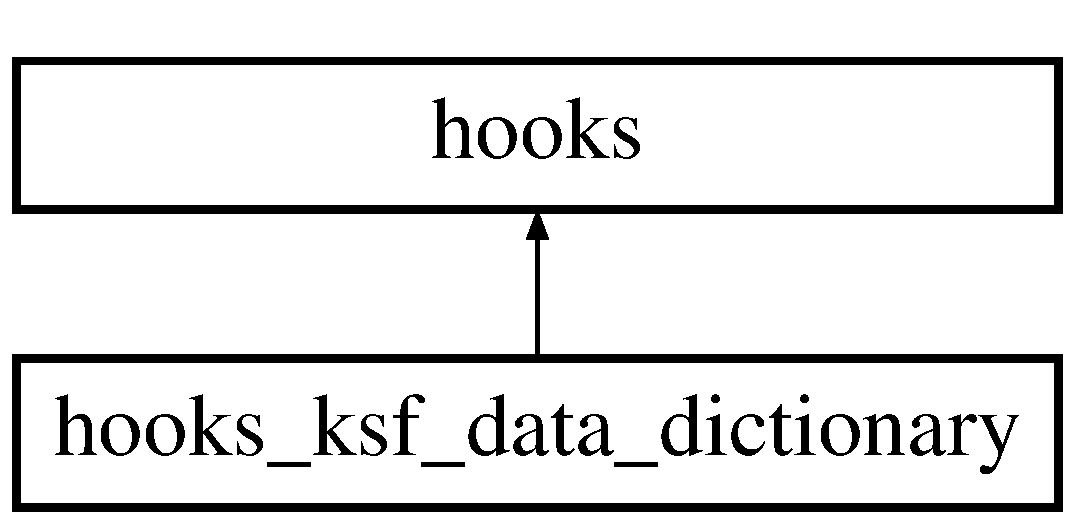
\includegraphics[height=2.000000cm]{d6/df1/classhooks__ksf__data__dictionary}
\end{center}
\end{figure}
\subsection*{Public Member Functions}
\begin{DoxyCompactItemize}
\item 
\hypertarget{classhooks__ksf__data__dictionary_a51c2d4fb996bbf3c60f37afe16adcbdb}{}\label{classhooks__ksf__data__dictionary_a51c2d4fb996bbf3c60f37afe16adcbdb} 
{\bfseries install\+\_\+options} (\$app)
\item 
\hypertarget{classhooks__ksf__data__dictionary_ab7c5be10650a64d4b2c52de979b052ba}{}\label{classhooks__ksf__data__dictionary_ab7c5be10650a64d4b2c52de979b052ba} 
{\bfseries install\+\_\+access} ()
\item 
\hypertarget{classhooks__ksf__data__dictionary_ac2a69e2e5f533cb83d115062f212181f}{}\label{classhooks__ksf__data__dictionary_ac2a69e2e5f533cb83d115062f212181f} 
{\bfseries db\+\_\+postwrite} (\&\$cart, \$trans\+\_\+type)
\item 
\hypertarget{classhooks__ksf__data__dictionary_a19fd428e932961cf2cb8423227a57ed9}{}\label{classhooks__ksf__data__dictionary_a19fd428e932961cf2cb8423227a57ed9} 
{\bfseries activate\+\_\+extension} (\$company, \$check\+\_\+only=true)
\item 
\hypertarget{classhooks__ksf__data__dictionary_afce221968539103514cc3b5f67ccbf64}{}\label{classhooks__ksf__data__dictionary_afce221968539103514cc3b5f67ccbf64} 
{\bfseries deactivate\+\_\+extension} (\$company, \$check\+\_\+only=true)
\end{DoxyCompactItemize}
\subsection*{Public Attributes}
\begin{DoxyCompactItemize}
\item 
\hypertarget{classhooks__ksf__data__dictionary_ab992bd3fc9279df2411ed79dca0e6f6d}{}\label{classhooks__ksf__data__dictionary_ab992bd3fc9279df2411ed79dca0e6f6d} 
{\bfseries \$module\+\_\+name} = \textquotesingle{}\hyperlink{classksf__data__dictionary}{ksf\+\_\+data\+\_\+dictionary}\textquotesingle{}
\end{DoxyCompactItemize}


The documentation for this class was generated from the following file\+:\begin{DoxyCompactItemize}
\item 
hooks.\+php\end{DoxyCompactItemize}

\hypertarget{classksf__data__dictionary}{}\section{ksf\+\_\+data\+\_\+dictionary Class Reference}
\label{classksf__data__dictionary}\index{ksf\+\_\+data\+\_\+dictionary@{ksf\+\_\+data\+\_\+dictionary}}
Inheritance diagram for ksf\+\_\+data\+\_\+dictionary\+:\begin{figure}[H]
\begin{center}
\leavevmode
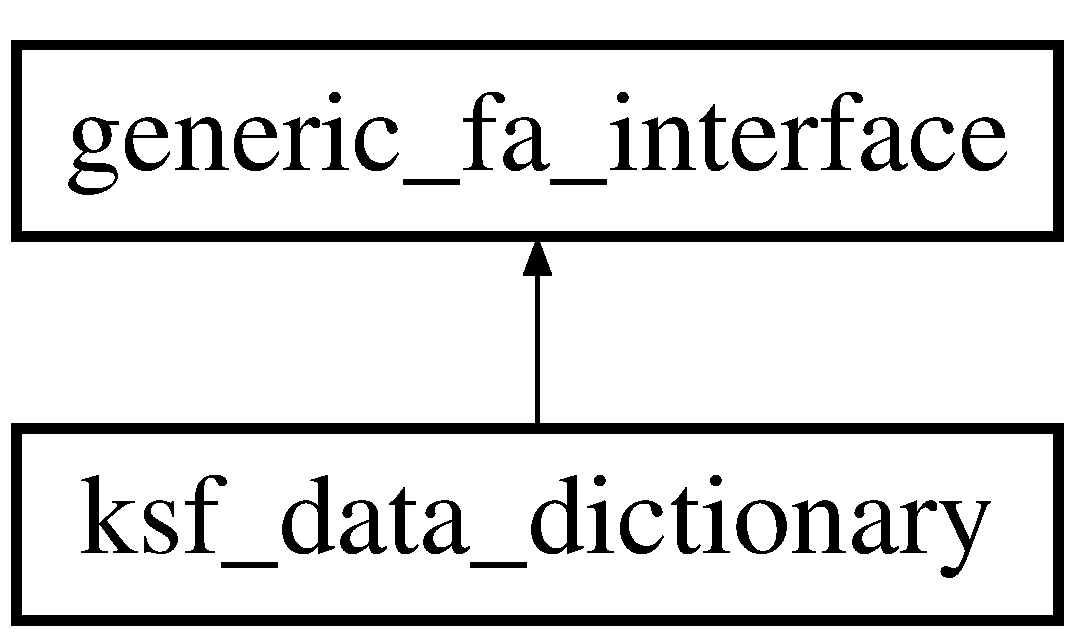
\includegraphics[height=2.000000cm]{d4/d83/classksf__data__dictionary}
\end{center}
\end{figure}
\subsection*{Public Member Functions}
\begin{DoxyCompactItemize}
\item 
\hypertarget{classksf__data__dictionary_acb25c29a1061b3a6d9e30c06fbb2c10e}{}\label{classksf__data__dictionary_acb25c29a1061b3a6d9e30c06fbb2c10e} 
{\bfseries \+\_\+\+\_\+construct} ( \$host, \$user, \$pass, \$database, \$pref\+\_\+tablename, \$ui\+\_\+caller)
\item 
\hypertarget{classksf__data__dictionary_a7c16a24545d7b021f36cbe8db1960240}{}\label{classksf__data__dictionary_a7c16a24545d7b021f36cbe8db1960240} 
{\bfseries define\+\_\+table} ()
\item 
\hyperlink{classksf__data__dictionary_af5a8a952ccf5cf307449559a8c0219b3}{fix\+\_\+stock\+\_\+id\+\_\+size} ()
\end{DoxyCompactItemize}
\subsection*{Public Attributes}
\begin{DoxyCompactItemize}
\item 
\hypertarget{classksf__data__dictionary_a073be682441a5cac9003e3b1d35add67}{}\label{classksf__data__dictionary_a073be682441a5cac9003e3b1d35add67} 
{\bfseries \$db}
\item 
\hypertarget{classksf__data__dictionary_ae9ffadd22abc35408de8169e195d9c60}{}\label{classksf__data__dictionary_ae9ffadd22abc35408de8169e195d9c60} 
{\bfseries \$ck}
\item 
\hypertarget{classksf__data__dictionary_acef5fa3bf3049242c863eefdd829f306}{}\label{classksf__data__dictionary_acef5fa3bf3049242c863eefdd829f306} 
{\bfseries \$cs}
\item 
\hypertarget{classksf__data__dictionary_a8f8039fa67a90e858eb3affbc8899f2c}{}\label{classksf__data__dictionary_a8f8039fa67a90e858eb3affbc8899f2c} 
{\bfseries \$server}
\item 
\hypertarget{classksf__data__dictionary_ad9cee0d471b634e5e231b3b2283fbd43}{}\label{classksf__data__dictionary_ad9cee0d471b634e5e231b3b2283fbd43} 
{\bfseries \$rest\+\_\+path}
\item 
\hypertarget{classksf__data__dictionary_a52e49c26728a76d726311d6ce6a4604e}{}\label{classksf__data__dictionary_a52e49c26728a76d726311d6ce6a4604e} 
{\bfseries \$environment}
\item 
\hypertarget{classksf__data__dictionary_ac5293f7337f3c456435a15fb3a36790b}{}\label{classksf__data__dictionary_ac5293f7337f3c456435a15fb3a36790b} 
{\bfseries \$debug}
\item 
\hypertarget{classksf__data__dictionary_a1897d718b0ce22d30ffc8d4a4eff0f05}{}\label{classksf__data__dictionary_a1897d718b0ce22d30ffc8d4a4eff0f05} 
{\bfseries \$alters\+\_\+needed}
\end{DoxyCompactItemize}


\subsection{Detailed Description}
data\+\_\+dictionary module \begin{DoxyVerb}Purpose of this module is to alter Front Accounting tables
so that column widths are large enough for the modules
we have added.

We will have a form to launch the table alters.

We will take an array of tables, their column name,
and the new sizes/attributes.

The form will launch an ALTER TABLES set of queries.
Probably should set it to be ATOMIC so that if an update
fails they are all rolled back.  However, fields too large
is less of a problem than too small.

Eventually I might add a table to store the alterations,
as well as a screen to populate the table.\end{DoxyVerb}


\hyperlink{classksf__data__dictionary}{ksf\+\_\+data\+\_\+dictionary} extends generic\+\_\+fa\+\_\+interface \begin{DoxyVerb}This class can be extended in a number of ways.
$this->alters_needed needs to have any field defining routine added since
it is called by the UI screen.

You could simply add a function and update alters_needed.

You can extend the class, creating a new function that defines the table.
You would also need to alter the UI class to find the extended class...

You could alter the routine fix_stock_id_size by adding more tables into the
array definition.

You could use this class and call $this->modify_table_column() with your own 
table definition.\end{DoxyVerb}
 

\subsection{Member Function Documentation}
\hypertarget{classksf__data__dictionary_af5a8a952ccf5cf307449559a8c0219b3}{}\label{classksf__data__dictionary_af5a8a952ccf5cf307449559a8c0219b3} 
\index{ksf\+\_\+data\+\_\+dictionary@{ksf\+\_\+data\+\_\+dictionary}!fix\+\_\+stock\+\_\+id\+\_\+size@{fix\+\_\+stock\+\_\+id\+\_\+size}}
\index{fix\+\_\+stock\+\_\+id\+\_\+size@{fix\+\_\+stock\+\_\+id\+\_\+size}!ksf\+\_\+data\+\_\+dictionary@{ksf\+\_\+data\+\_\+dictionary}}
\subsubsection{\texorpdfstring{fix\+\_\+stock\+\_\+id\+\_\+size()}{fix\_stock\_id\_size()}}
{\footnotesize\ttfamily ksf\+\_\+data\+\_\+dictionary\+::fix\+\_\+stock\+\_\+id\+\_\+size (\begin{DoxyParamCaption}{ }\end{DoxyParamCaption})}

fix\+\_\+stock\+\_\+id\+\_\+size \begin{DoxyVerb}Because of variation products (have attributes such as size and color) where 
everything else is the same, we want mostly human readable SKUs so that we
can easily type them in without having to hunt for them.  This requires longer
SKU lengths.  Default of 20 doesn't work for us anymore.

This function alters all of the tables (that we know of) to have the longer
length.  The Length is defined in an include file where we are putting
lengths so we can do this to other tables as needed too.\end{DoxyVerb}
 

The documentation for this class was generated from the following file\+:\begin{DoxyCompactItemize}
\item 
class.\+ksf\+\_\+data\+\_\+dictionary.\+php\end{DoxyCompactItemize}

\hypertarget{classksf__data__dictionary__ui}{}\section{ksf\+\_\+data\+\_\+dictionary\+\_\+ui Class Reference}
\label{classksf__data__dictionary__ui}\index{ksf\+\_\+data\+\_\+dictionary\+\_\+ui@{ksf\+\_\+data\+\_\+dictionary\+\_\+ui}}
Inheritance diagram for ksf\+\_\+data\+\_\+dictionary\+\_\+ui\+:\begin{figure}[H]
\begin{center}
\leavevmode
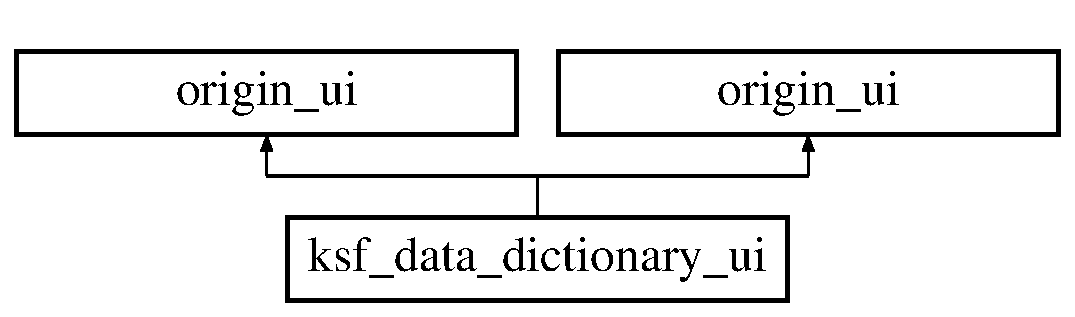
\includegraphics[height=2.000000cm]{d0/d52/classksf__data__dictionary__ui}
\end{center}
\end{figure}
\subsection*{Public Member Functions}
\begin{DoxyCompactItemize}
\item 
\hypertarget{classksf__data__dictionary__ui_a2e77b829675b895057a095e1f848ddcf}{}\label{classksf__data__dictionary__ui_a2e77b829675b895057a095e1f848ddcf} 
{\bfseries \+\_\+\+\_\+construct} ( \$host, \$user, \$pass, \$database, \$pref\+\_\+tablename, \$caller=null)
\item 
\hyperlink{classksf__data__dictionary__ui_a0a29d77c9427ed3b3c76926f3810fab5}{is\+\_\+installed} ()
\item 
\hyperlink{classksf__data__dictionary__ui_a718a382712dc59fe7541a6dc77c5d1c0}{run} ()
\item 
\hyperlink{classksf__data__dictionary__ui_a3c01247145824cdf9ad196e2c1e1ad80}{show\+\_\+config\+\_\+form} ()
\item 
\hyperlink{classksf__data__dictionary__ui_ac0d782167419454b7bbba4a8aa3e98e1}{create\+\_\+data\+\_\+dictionary\+\_\+form} ()
\item 
\hypertarget{classksf__data__dictionary__ui_a40244068b94acbc83667a3db70a65dd8}{}\label{classksf__data__dictionary__ui_a40244068b94acbc83667a3db70a65dd8} 
{\bfseries init\+\_\+tables\+\_\+complete\+\_\+form} ()
\item 
\hypertarget{classksf__data__dictionary__ui_afbff679af2f43df46442270aa8684b88}{}\label{classksf__data__dictionary__ui_afbff679af2f43df46442270aa8684b88} 
{\bfseries created\+\_\+data\+\_\+dictionary\+\_\+form} ()
\item 
\hypertarget{classksf__data__dictionary__ui_ae72e2830a5968177c20c70884cc78e54}{}\label{classksf__data__dictionary__ui_ae72e2830a5968177c20c70884cc78e54} 
{\bfseries init\+\_\+tables\+\_\+form} ()
\item 
\hypertarget{classksf__data__dictionary__ui_a50ce94fab9edff56f02cb2cc5f64e8d5}{}\label{classksf__data__dictionary__ui_a50ce94fab9edff56f02cb2cc5f64e8d5} 
{\bfseries alter\+\_\+tables\+\_\+form} ()
\item 
\hypertarget{classksf__data__dictionary__ui_aec7ec64ecde5afe4ff026b0c2d4dea12}{}\label{classksf__data__dictionary__ui_aec7ec64ecde5afe4ff026b0c2d4dea12} 
{\bfseries alter\+\_\+tables\+\_\+complete\+\_\+form} ()
\item 
\hypertarget{classksf__data__dictionary__ui_a2e77b829675b895057a095e1f848ddcf}{}\label{classksf__data__dictionary__ui_a2e77b829675b895057a095e1f848ddcf} 
{\bfseries \+\_\+\+\_\+construct} ( \$host, \$user, \$pass, \$database, \$pref\+\_\+tablename, \$caller=null)
\item 
\hyperlink{classksf__data__dictionary__ui_a0a29d77c9427ed3b3c76926f3810fab5}{is\+\_\+installed} ()
\item 
\hyperlink{classksf__data__dictionary__ui_a718a382712dc59fe7541a6dc77c5d1c0}{run} ()
\item 
\hyperlink{classksf__data__dictionary__ui_a3c01247145824cdf9ad196e2c1e1ad80}{show\+\_\+config\+\_\+form} ()
\item 
\hyperlink{classksf__data__dictionary__ui_ac0d782167419454b7bbba4a8aa3e98e1}{create\+\_\+data\+\_\+dictionary\+\_\+form} ()
\item 
\hypertarget{classksf__data__dictionary__ui_a40244068b94acbc83667a3db70a65dd8}{}\label{classksf__data__dictionary__ui_a40244068b94acbc83667a3db70a65dd8} 
{\bfseries init\+\_\+tables\+\_\+complete\+\_\+form} ()
\item 
\hypertarget{classksf__data__dictionary__ui_afbff679af2f43df46442270aa8684b88}{}\label{classksf__data__dictionary__ui_afbff679af2f43df46442270aa8684b88} 
{\bfseries created\+\_\+data\+\_\+dictionary\+\_\+form} ()
\item 
\hypertarget{classksf__data__dictionary__ui_ae72e2830a5968177c20c70884cc78e54}{}\label{classksf__data__dictionary__ui_ae72e2830a5968177c20c70884cc78e54} 
{\bfseries init\+\_\+tables\+\_\+form} ()
\item 
\hypertarget{classksf__data__dictionary__ui_a50ce94fab9edff56f02cb2cc5f64e8d5}{}\label{classksf__data__dictionary__ui_a50ce94fab9edff56f02cb2cc5f64e8d5} 
{\bfseries alter\+\_\+tables\+\_\+form} ()
\item 
\hypertarget{classksf__data__dictionary__ui_aec7ec64ecde5afe4ff026b0c2d4dea12}{}\label{classksf__data__dictionary__ui_aec7ec64ecde5afe4ff026b0c2d4dea12} 
{\bfseries alter\+\_\+tables\+\_\+complete\+\_\+form} ()
\end{DoxyCompactItemize}
\subsection*{Public Attributes}
\begin{DoxyCompactItemize}
\item 
\hypertarget{classksf__data__dictionary__ui_a5b4d8968def8c3345673618d845d9004}{}\label{classksf__data__dictionary__ui_a5b4d8968def8c3345673618d845d9004} 
\hyperlink{classksf__data__dictionary__ui_a5b4d8968def8c3345673618d845d9004}{\$caller}
\begin{DoxyCompactList}\small\item\em which class called us. \end{DoxyCompactList}\item 
\hypertarget{classksf__data__dictionary__ui_a44e50c035641328fa22cedc0c0d0b9dc}{}\label{classksf__data__dictionary__ui_a44e50c035641328fa22cedc0c0d0b9dc} 
{\bfseries \$data\+\_\+dictionary}
\end{DoxyCompactItemize}


\subsection{Detailed Description}
data\+\_\+dictionary module UI \begin{DoxyVerb}Purpose of this module is to alter Front Accounting tables
so that column widths are large enough for the modules
we have added.

We will have a form to launch the table alters.

We will take an array of tables, their column name,
and the new sizes/attributes.

The form will launch an ALTER TABLES set of queries.
Probably should set it to be ATOMIC so that if an update
fails they are all rolled back.  However, fields too large
is less of a problem than too small.\end{DoxyVerb}
 

\subsection{Member Function Documentation}
\hypertarget{classksf__data__dictionary__ui_ac0d782167419454b7bbba4a8aa3e98e1}{}\label{classksf__data__dictionary__ui_ac0d782167419454b7bbba4a8aa3e98e1} 
\index{ksf\+\_\+data\+\_\+dictionary\+\_\+ui@{ksf\+\_\+data\+\_\+dictionary\+\_\+ui}!create\+\_\+data\+\_\+dictionary\+\_\+form@{create\+\_\+data\+\_\+dictionary\+\_\+form}}
\index{create\+\_\+data\+\_\+dictionary\+\_\+form@{create\+\_\+data\+\_\+dictionary\+\_\+form}!ksf\+\_\+data\+\_\+dictionary\+\_\+ui@{ksf\+\_\+data\+\_\+dictionary\+\_\+ui}}
\subsubsection{\texorpdfstring{create\+\_\+data\+\_\+dictionary\+\_\+form()}{create\_data\_dictionary\_form()}\hspace{0.1cm}{\footnotesize\ttfamily [1/2]}}
{\footnotesize\ttfamily ksf\+\_\+data\+\_\+dictionary\+\_\+ui\+::create\+\_\+data\+\_\+dictionary\+\_\+form (\begin{DoxyParamCaption}{ }\end{DoxyParamCaption})}

create\+\_\+data\+\_\+dictionary\+\_\+form

Display a form on screen for generating a data\+\_\+dictionary \hypertarget{classksf__data__dictionary__ui_ac0d782167419454b7bbba4a8aa3e98e1}{}\label{classksf__data__dictionary__ui_ac0d782167419454b7bbba4a8aa3e98e1} 
\index{ksf\+\_\+data\+\_\+dictionary\+\_\+ui@{ksf\+\_\+data\+\_\+dictionary\+\_\+ui}!create\+\_\+data\+\_\+dictionary\+\_\+form@{create\+\_\+data\+\_\+dictionary\+\_\+form}}
\index{create\+\_\+data\+\_\+dictionary\+\_\+form@{create\+\_\+data\+\_\+dictionary\+\_\+form}!ksf\+\_\+data\+\_\+dictionary\+\_\+ui@{ksf\+\_\+data\+\_\+dictionary\+\_\+ui}}
\subsubsection{\texorpdfstring{create\+\_\+data\+\_\+dictionary\+\_\+form()}{create\_data\_dictionary\_form()}\hspace{0.1cm}{\footnotesize\ttfamily [2/2]}}
{\footnotesize\ttfamily ksf\+\_\+data\+\_\+dictionary\+\_\+ui\+::create\+\_\+data\+\_\+dictionary\+\_\+form (\begin{DoxyParamCaption}{ }\end{DoxyParamCaption})}

create\+\_\+data\+\_\+dictionary\+\_\+form

Display a form on screen for generating a data\+\_\+dictionary \hypertarget{classksf__data__dictionary__ui_a0a29d77c9427ed3b3c76926f3810fab5}{}\label{classksf__data__dictionary__ui_a0a29d77c9427ed3b3c76926f3810fab5} 
\index{ksf\+\_\+data\+\_\+dictionary\+\_\+ui@{ksf\+\_\+data\+\_\+dictionary\+\_\+ui}!is\+\_\+installed@{is\+\_\+installed}}
\index{is\+\_\+installed@{is\+\_\+installed}!ksf\+\_\+data\+\_\+dictionary\+\_\+ui@{ksf\+\_\+data\+\_\+dictionary\+\_\+ui}}
\subsubsection{\texorpdfstring{is\+\_\+installed()}{is\_installed()}\hspace{0.1cm}{\footnotesize\ttfamily [1/2]}}
{\footnotesize\ttfamily ksf\+\_\+data\+\_\+dictionary\+\_\+ui\+::is\+\_\+installed (\begin{DoxyParamCaption}{ }\end{DoxyParamCaption})}

is\+\_\+installed \hypertarget{classksf__data__dictionary__ui_a0a29d77c9427ed3b3c76926f3810fab5}{}\label{classksf__data__dictionary__ui_a0a29d77c9427ed3b3c76926f3810fab5} 
\index{ksf\+\_\+data\+\_\+dictionary\+\_\+ui@{ksf\+\_\+data\+\_\+dictionary\+\_\+ui}!is\+\_\+installed@{is\+\_\+installed}}
\index{is\+\_\+installed@{is\+\_\+installed}!ksf\+\_\+data\+\_\+dictionary\+\_\+ui@{ksf\+\_\+data\+\_\+dictionary\+\_\+ui}}
\subsubsection{\texorpdfstring{is\+\_\+installed()}{is\_installed()}\hspace{0.1cm}{\footnotesize\ttfamily [2/2]}}
{\footnotesize\ttfamily ksf\+\_\+data\+\_\+dictionary\+\_\+ui\+::is\+\_\+installed (\begin{DoxyParamCaption}{ }\end{DoxyParamCaption})}

is\+\_\+installed \hypertarget{classksf__data__dictionary__ui_a718a382712dc59fe7541a6dc77c5d1c0}{}\label{classksf__data__dictionary__ui_a718a382712dc59fe7541a6dc77c5d1c0} 
\index{ksf\+\_\+data\+\_\+dictionary\+\_\+ui@{ksf\+\_\+data\+\_\+dictionary\+\_\+ui}!run@{run}}
\index{run@{run}!ksf\+\_\+data\+\_\+dictionary\+\_\+ui@{ksf\+\_\+data\+\_\+dictionary\+\_\+ui}}
\subsubsection{\texorpdfstring{run()}{run()}\hspace{0.1cm}{\footnotesize\ttfamily [1/2]}}
{\footnotesize\ttfamily ksf\+\_\+data\+\_\+dictionary\+\_\+ui\+::run (\begin{DoxyParamCaption}{ }\end{DoxyParamCaption})}

run \hypertarget{classksf__data__dictionary__ui_a718a382712dc59fe7541a6dc77c5d1c0}{}\label{classksf__data__dictionary__ui_a718a382712dc59fe7541a6dc77c5d1c0} 
\index{ksf\+\_\+data\+\_\+dictionary\+\_\+ui@{ksf\+\_\+data\+\_\+dictionary\+\_\+ui}!run@{run}}
\index{run@{run}!ksf\+\_\+data\+\_\+dictionary\+\_\+ui@{ksf\+\_\+data\+\_\+dictionary\+\_\+ui}}
\subsubsection{\texorpdfstring{run()}{run()}\hspace{0.1cm}{\footnotesize\ttfamily [2/2]}}
{\footnotesize\ttfamily ksf\+\_\+data\+\_\+dictionary\+\_\+ui\+::run (\begin{DoxyParamCaption}{ }\end{DoxyParamCaption})}

run \hypertarget{classksf__data__dictionary__ui_a3c01247145824cdf9ad196e2c1e1ad80}{}\label{classksf__data__dictionary__ui_a3c01247145824cdf9ad196e2c1e1ad80} 
\index{ksf\+\_\+data\+\_\+dictionary\+\_\+ui@{ksf\+\_\+data\+\_\+dictionary\+\_\+ui}!show\+\_\+config\+\_\+form@{show\+\_\+config\+\_\+form}}
\index{show\+\_\+config\+\_\+form@{show\+\_\+config\+\_\+form}!ksf\+\_\+data\+\_\+dictionary\+\_\+ui@{ksf\+\_\+data\+\_\+dictionary\+\_\+ui}}
\subsubsection{\texorpdfstring{show\+\_\+config\+\_\+form()}{show\_config\_form()}\hspace{0.1cm}{\footnotesize\ttfamily [1/2]}}
{\footnotesize\ttfamily ksf\+\_\+data\+\_\+dictionary\+\_\+ui\+::show\+\_\+config\+\_\+form (\begin{DoxyParamCaption}{ }\end{DoxyParamCaption})}

Inherited \hyperlink{classksf__data__dictionary__ui_a3c01247145824cdf9ad196e2c1e1ad80}{show\+\_\+config\+\_\+form()} \hypertarget{classksf__data__dictionary__ui_a3c01247145824cdf9ad196e2c1e1ad80}{}\label{classksf__data__dictionary__ui_a3c01247145824cdf9ad196e2c1e1ad80} 
\index{ksf\+\_\+data\+\_\+dictionary\+\_\+ui@{ksf\+\_\+data\+\_\+dictionary\+\_\+ui}!show\+\_\+config\+\_\+form@{show\+\_\+config\+\_\+form}}
\index{show\+\_\+config\+\_\+form@{show\+\_\+config\+\_\+form}!ksf\+\_\+data\+\_\+dictionary\+\_\+ui@{ksf\+\_\+data\+\_\+dictionary\+\_\+ui}}
\subsubsection{\texorpdfstring{show\+\_\+config\+\_\+form()}{show\_config\_form()}\hspace{0.1cm}{\footnotesize\ttfamily [2/2]}}
{\footnotesize\ttfamily ksf\+\_\+data\+\_\+dictionary\+\_\+ui\+::show\+\_\+config\+\_\+form (\begin{DoxyParamCaption}{ }\end{DoxyParamCaption})}

Inherited \hyperlink{classksf__data__dictionary__ui_a3c01247145824cdf9ad196e2c1e1ad80}{show\+\_\+config\+\_\+form()} 

The documentation for this class was generated from the following files\+:\begin{DoxyCompactItemize}
\item 
class.\+ksf\+\_\+data\+\_\+dictionary\+\_\+ui.\+bak.\+php\item 
class.\+ksf\+\_\+data\+\_\+dictionary\+\_\+ui.\+php\end{DoxyCompactItemize}

\hypertarget{classorigin__ui2}{}\section{origin\+\_\+ui2 Class Reference}
\label{classorigin__ui2}\index{origin\+\_\+ui2@{origin\+\_\+ui2}}
Inheritance diagram for origin\+\_\+ui2\+:\begin{figure}[H]
\begin{center}
\leavevmode
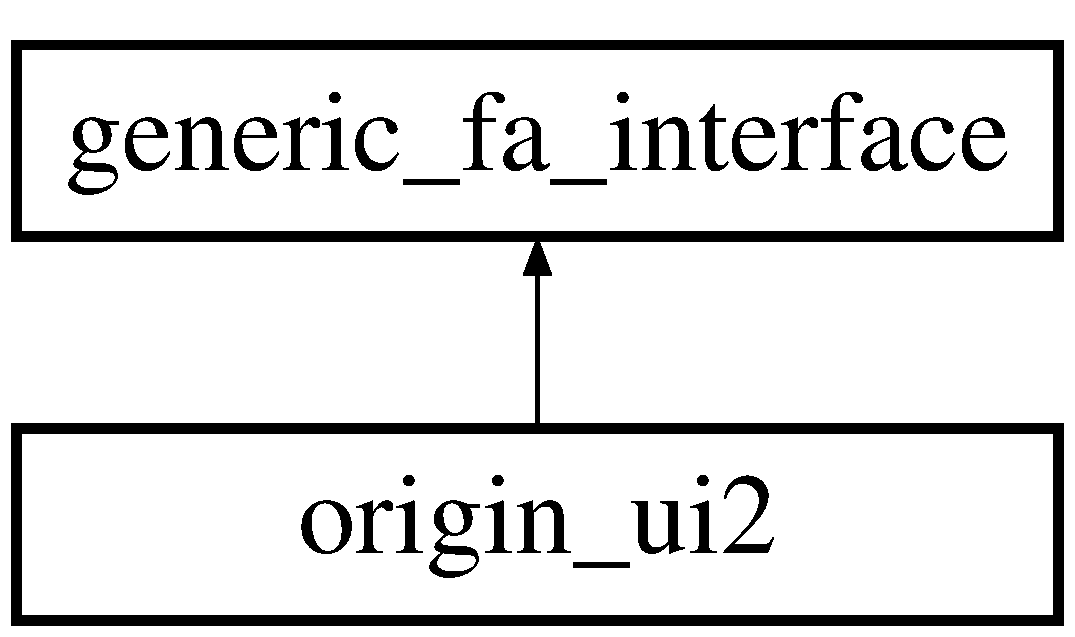
\includegraphics[height=2.000000cm]{d1/db2/classorigin__ui2}
\end{center}
\end{figure}
\subsection*{Public Member Functions}
\begin{DoxyCompactItemize}
\item 
\hyperlink{classorigin__ui2_a503ff6b0a877a4c85fb08f75b81b630e}{\+\_\+\+\_\+construct} ( \$client)
\item 
\hyperlink{classorigin__ui2_ac79b126fb01d3f54d2507c860564655d}{fields\+\_\+array2var} ()
\item 
\hyperlink{classorigin__ui2_a59694769d976755cce9b17e83780bacf}{in\+\_\+table\+\_\+display} ( \$field\+\_\+array)
\item 
\hyperlink{classorigin__ui2_a5bd82705d8ecde76f63e77920b8f8e89}{call\+\_\+table} ( \$action, \$msg)
\end{DoxyCompactItemize}


\subsection{Detailed Description}
class origin\+\_\+ui

Common processes for UI classes

Functions\+: fields\+\_\+array2var in\+\_\+table\+\_\+display call\+\_\+table Inherited\+: (not guaranteed to be complete due to changes in inherited class(es) 

\subsection{Constructor \& Destructor Documentation}
\hypertarget{classorigin__ui2_a503ff6b0a877a4c85fb08f75b81b630e}{}\label{classorigin__ui2_a503ff6b0a877a4c85fb08f75b81b630e} 
\index{origin\+\_\+ui2@{origin\+\_\+ui2}!\+\_\+\+\_\+construct@{\+\_\+\+\_\+construct}}
\index{\+\_\+\+\_\+construct@{\+\_\+\+\_\+construct}!origin\+\_\+ui2@{origin\+\_\+ui2}}
\subsubsection{\texorpdfstring{\+\_\+\+\_\+construct()}{\_\_construct()}}
{\footnotesize\ttfamily origin\+\_\+ui2\+::\+\_\+\+\_\+construct (\begin{DoxyParamCaption}\item[{}]{\$client }\end{DoxyParamCaption})}


\begin{DoxyParams}{Parameters}
{\em object} & client object needing values set \\
\hline
\end{DoxyParams}


\subsection{Member Function Documentation}
\hypertarget{classorigin__ui2_a5bd82705d8ecde76f63e77920b8f8e89}{}\label{classorigin__ui2_a5bd82705d8ecde76f63e77920b8f8e89} 
\index{origin\+\_\+ui2@{origin\+\_\+ui2}!call\+\_\+table@{call\+\_\+table}}
\index{call\+\_\+table@{call\+\_\+table}!origin\+\_\+ui2@{origin\+\_\+ui2}}
\subsubsection{\texorpdfstring{call\+\_\+table()}{call\_table()}}
{\footnotesize\ttfamily origin\+\_\+ui2\+::call\+\_\+table (\begin{DoxyParamCaption}\item[{}]{\$action,  }\item[{}]{\$msg }\end{DoxyParamCaption})}

call\+\_\+table \begin{DoxyVerb}Puts a table on the screen with a button
to act as a "Are you sure" type of screen
so that the user has to init the action.
\end{DoxyVerb}



\begin{DoxyParams}{Parameters}
{\em action} & routine (next screen) to call \\
\hline
{\em msg} & the message to be displayed on the button to push \\
\hline
\end{DoxyParams}
\begin{DoxyReturn}{Returns}
N\+O\+T\+H\+I\+NG 
\end{DoxyReturn}
\hypertarget{classorigin__ui2_ac79b126fb01d3f54d2507c860564655d}{}\label{classorigin__ui2_ac79b126fb01d3f54d2507c860564655d} 
\index{origin\+\_\+ui2@{origin\+\_\+ui2}!fields\+\_\+array2var@{fields\+\_\+array2var}}
\index{fields\+\_\+array2var@{fields\+\_\+array2var}!origin\+\_\+ui2@{origin\+\_\+ui2}}
\subsubsection{\texorpdfstring{fields\+\_\+array2var()}{fields\_array2var()}}
{\footnotesize\ttfamily origin\+\_\+ui2\+::fields\+\_\+array2var (\begin{DoxyParamCaption}{ }\end{DoxyParamCaption})}

fields\+\_\+array2var Take the data out of P\+O\+ST variables and put them into the variables defined as table columns (fields\+\_\+array)

\begin{DoxyVerb}@returns int count of fields set\end{DoxyVerb}
 \hypertarget{classorigin__ui2_a59694769d976755cce9b17e83780bacf}{}\label{classorigin__ui2_a59694769d976755cce9b17e83780bacf} 
\index{origin\+\_\+ui2@{origin\+\_\+ui2}!in\+\_\+table\+\_\+display@{in\+\_\+table\+\_\+display}}
\index{in\+\_\+table\+\_\+display@{in\+\_\+table\+\_\+display}!origin\+\_\+ui2@{origin\+\_\+ui2}}
\subsubsection{\texorpdfstring{in\+\_\+table\+\_\+display()}{in\_table\_display()}}
{\footnotesize\ttfamily origin\+\_\+ui2\+::in\+\_\+table\+\_\+display (\begin{DoxyParamCaption}\item[{}]{\$field\+\_\+array }\end{DoxyParamCaption})}

in\+\_\+table\+\_\+display


\begin{DoxyParams}{Parameters}
{\em array} & display on the screen, within a table, 1 row as specified by the array \\
\hline
\end{DoxyParams}


The documentation for this class was generated from the following file\+:\begin{DoxyCompactItemize}
\item 
class.\+ksf\+\_\+data\+\_\+dictionary\+\_\+ui.\+bak.\+php\end{DoxyCompactItemize}

%--- End generated contents ---

% Index
\backmatter
\newpage
\phantomsection
\clearemptydoublepage
\addcontentsline{toc}{chapter}{Index}
\printindex

\end{document}
